\chapter{Destructive 3D phenotyping pipeline}

\section{Introduction}

Estimating the plant phenotypes accurately and efficiently can help to bridge the gap between genotype and phenotype. The traditional phenotyping measurement is time-consuming, laborious, and often not accurate. Although several authors have developed 2D image-based phenotyping methods which are more efficient, non-destructive, and have higher throughput \citep{yang_greenness_2015,guo_easypcc_2017,zou_broccoli_2019}, these approaches are unable to describe the plant 3D structure due to the occlusion and dimension loss when projecting onto the 2D plane. As a result, it produces inaccuracies and uncertainties for advanced phenotyping applications.

To overcome the drawbacks of 2D image-based phenotyping, several studies have paid attention to 3D approaches. \citet{paulus_measuring_2019} and \citet{kochi_introduction_2021} have summarized the current approaches to obtain 3D plant models, and a large number of studies have chosen the 3D reconstruction by photogrammetry using common RGB cameras due to the low device cost \citep{xiao_estimating_2021,zermas_3d_2020,zhang_estimating_2016}. The key idea of sfm, was taking images from different angle views and calculating their relative positions to the object.

% the key idea of sfm, and the classes of sfm


\begin{figure}[htb]
  \begin{center}
    \resizebox{\textwidth}{!}{
      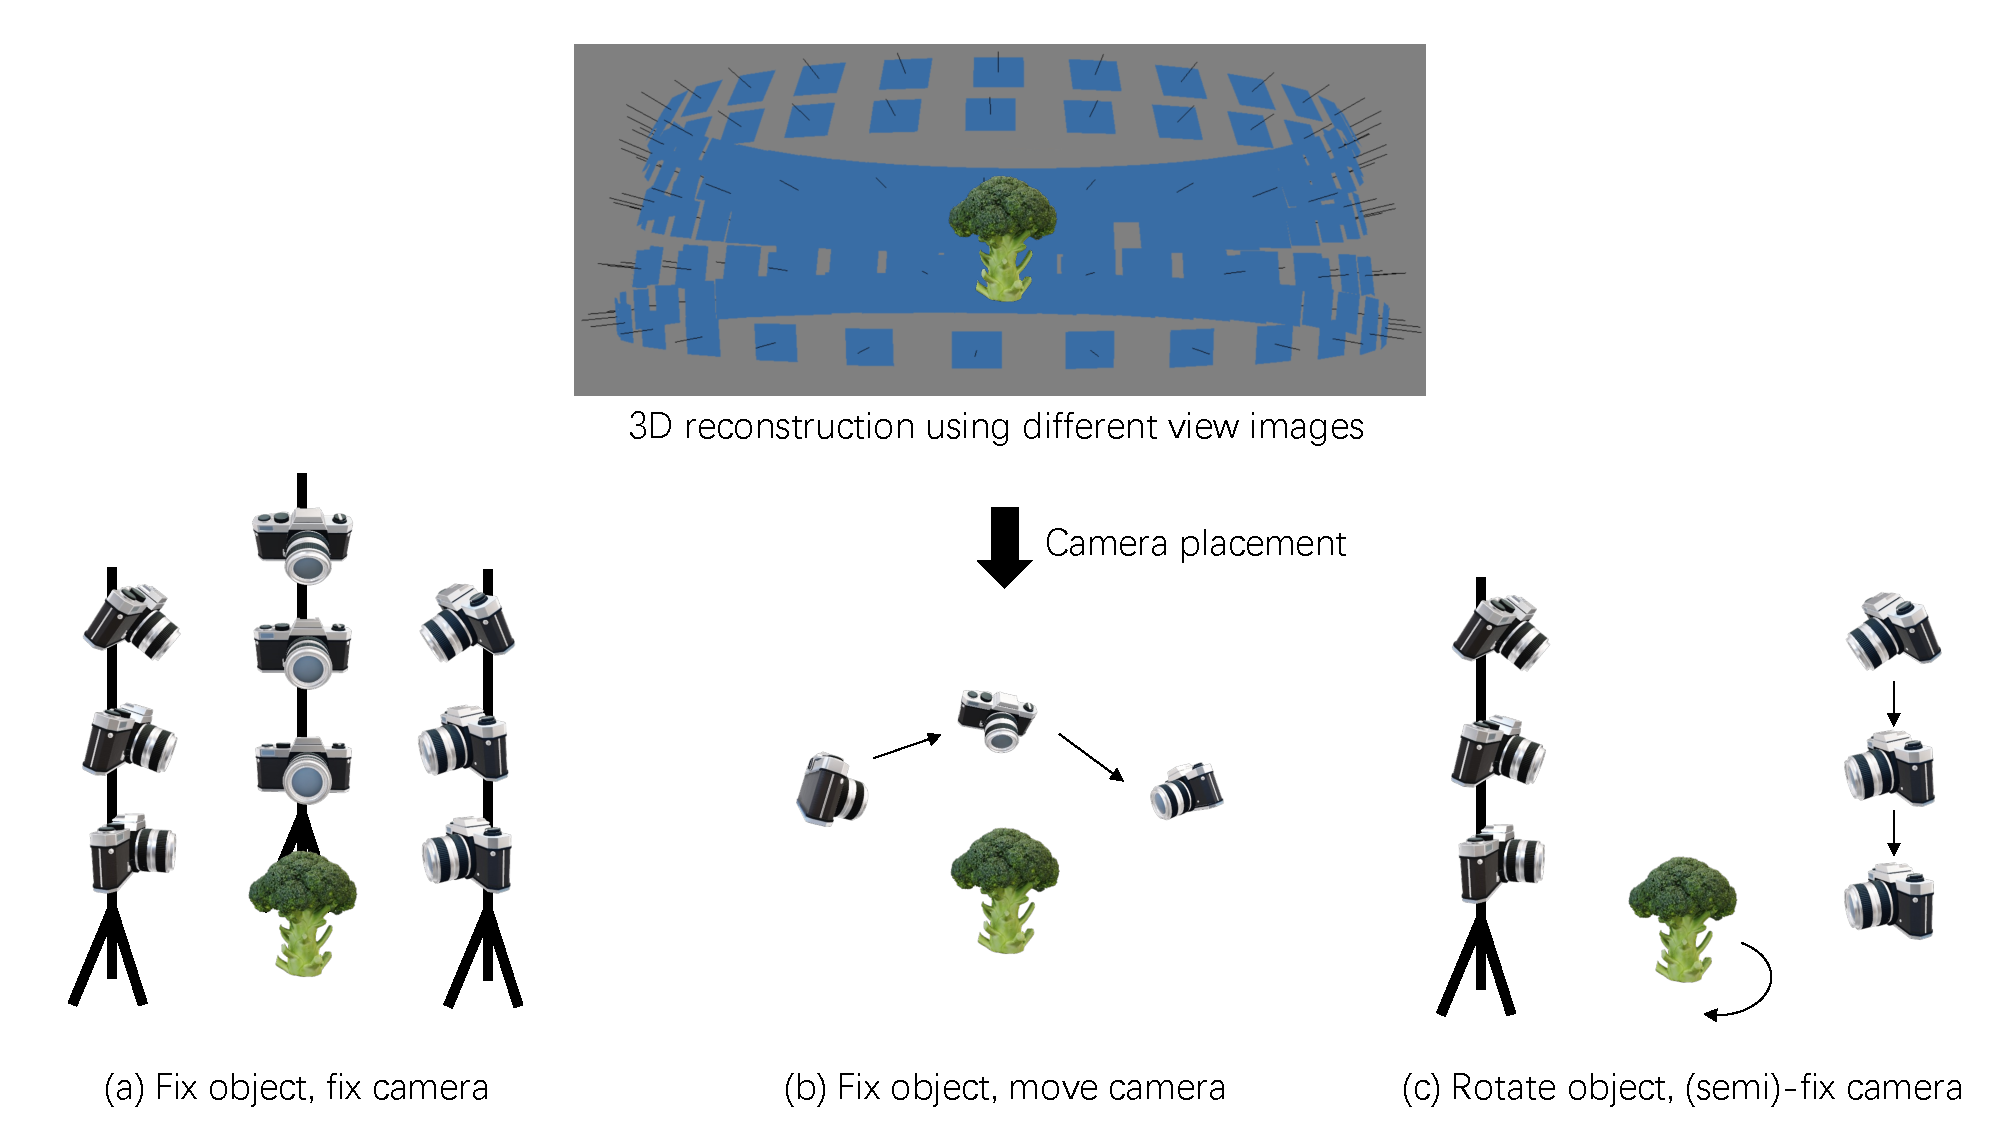
\includegraphics{figures/des/sfm_types.pdf}
    }
  \end{center}
  \caption[Current photogrammetry (3D reconstruction) methods and challenges]{
    The current photogrammetry (3D reconstruction) methods and challenges; (a-c) the current image acquisition approaches (a) fixing the object and taking images using multiple fixed cameras at the same time, also called forward intersection; (b) fixing the object but taking images by using a moved camera, also called backward resection; and (c) rotating the object and taking images using fewer multiple fixed cameras, or a camera fixed at different locations for each rotation. The challenges of current approaches: (d) the limited view angles of current image occlusion approaches has visual dead area, which will cause incomplete plant 3D models; and (e) the difficulties to segment foreground (plant) area in the image preprocessing.
  }
  \label{fig:des1}
\end{figure}


\section{Methods and Materials}

\subsection{Plant 3D model acquisition}

% plant materials, the information for fields and selective sampling

\subsubsection{Imaging device}

% figure2: 3D reconstruction devices
\begin{figure}[htb]
  \begin{center}
    \resizebox{\textwidth}{!}{
      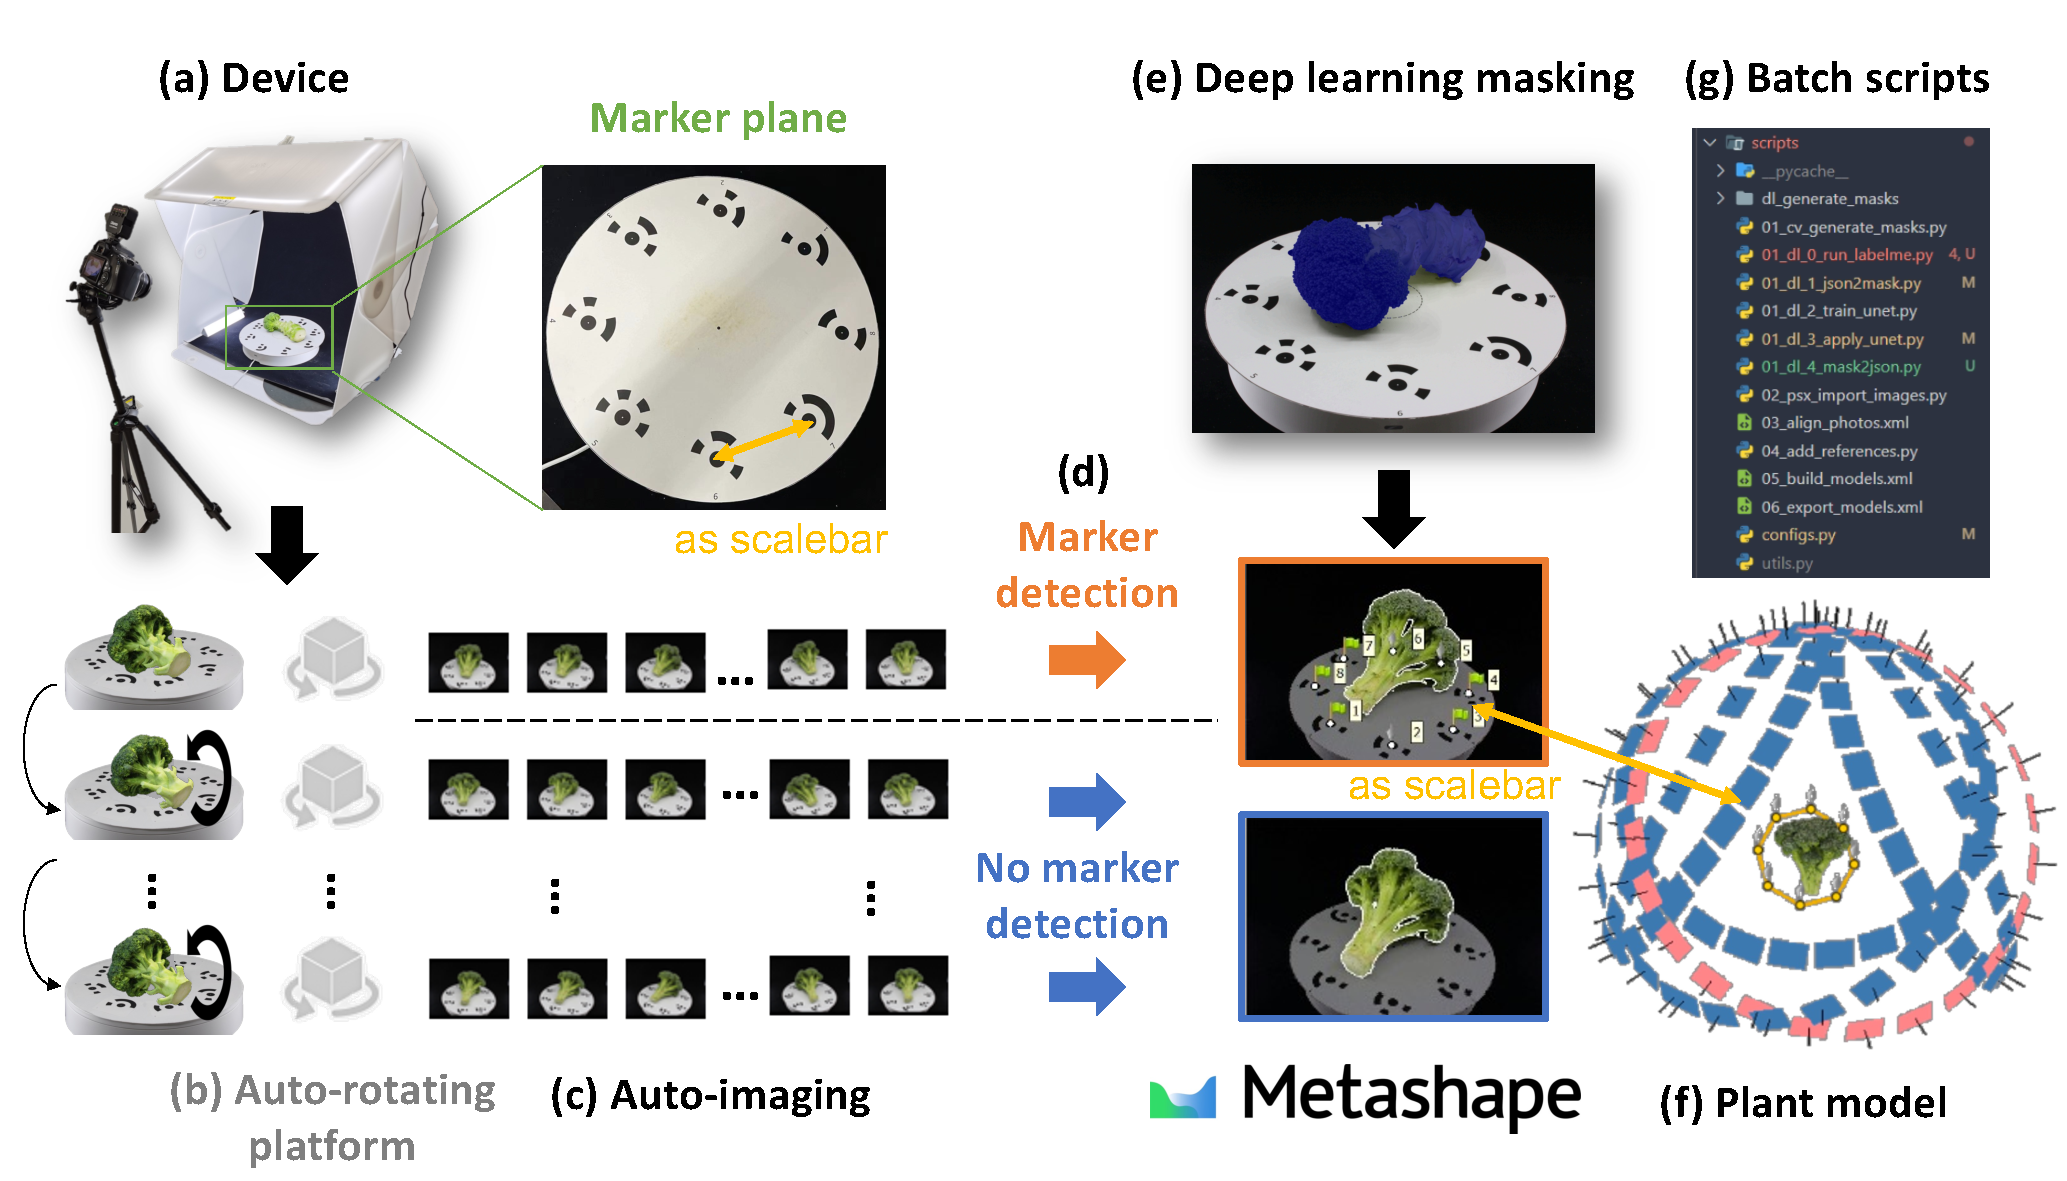
\includegraphics{figures/des/img_recons.pdf}
    }
  \end{center}
  \caption[The plant 3D model reconstruction workflow]{
    The Plant 3D model reconstruction workflow; (a) devices for taking plant images, with a marker plane used as scalebar references; (b) an automatic horizontal rotating platform, which can rotate at a given angle and then stop for a short interval for image taking. The vertical rotation of plants (flip) requires manual operation; (c) different photographic perspectives images taken by the infrared signal auto-imaging system; (d) partial marker detection to avoid misleading image alignment, where only markers on one rotating image group (orange) are detected and not on the others (blue); (e) plant part segmentation using deep learning; (f) the final 3D plant model produced by Metashape; and (g) the scripts for batch processing a large number of plants.
  }
  \label{fig:des_img_recons}
\end{figure}

\subsubsection{Image preprocessing}



\subsubsection{Batch 3D reconstruction}

% marker detection for one round and ignore for others

% the batch preprocessing 

\subsection{Phenotypic traits extraction}

% figure3: general workflow
\begin{figure}[htbp!]
  \begin{center}
    \resizebox{0.9\textwidth}{!}{
      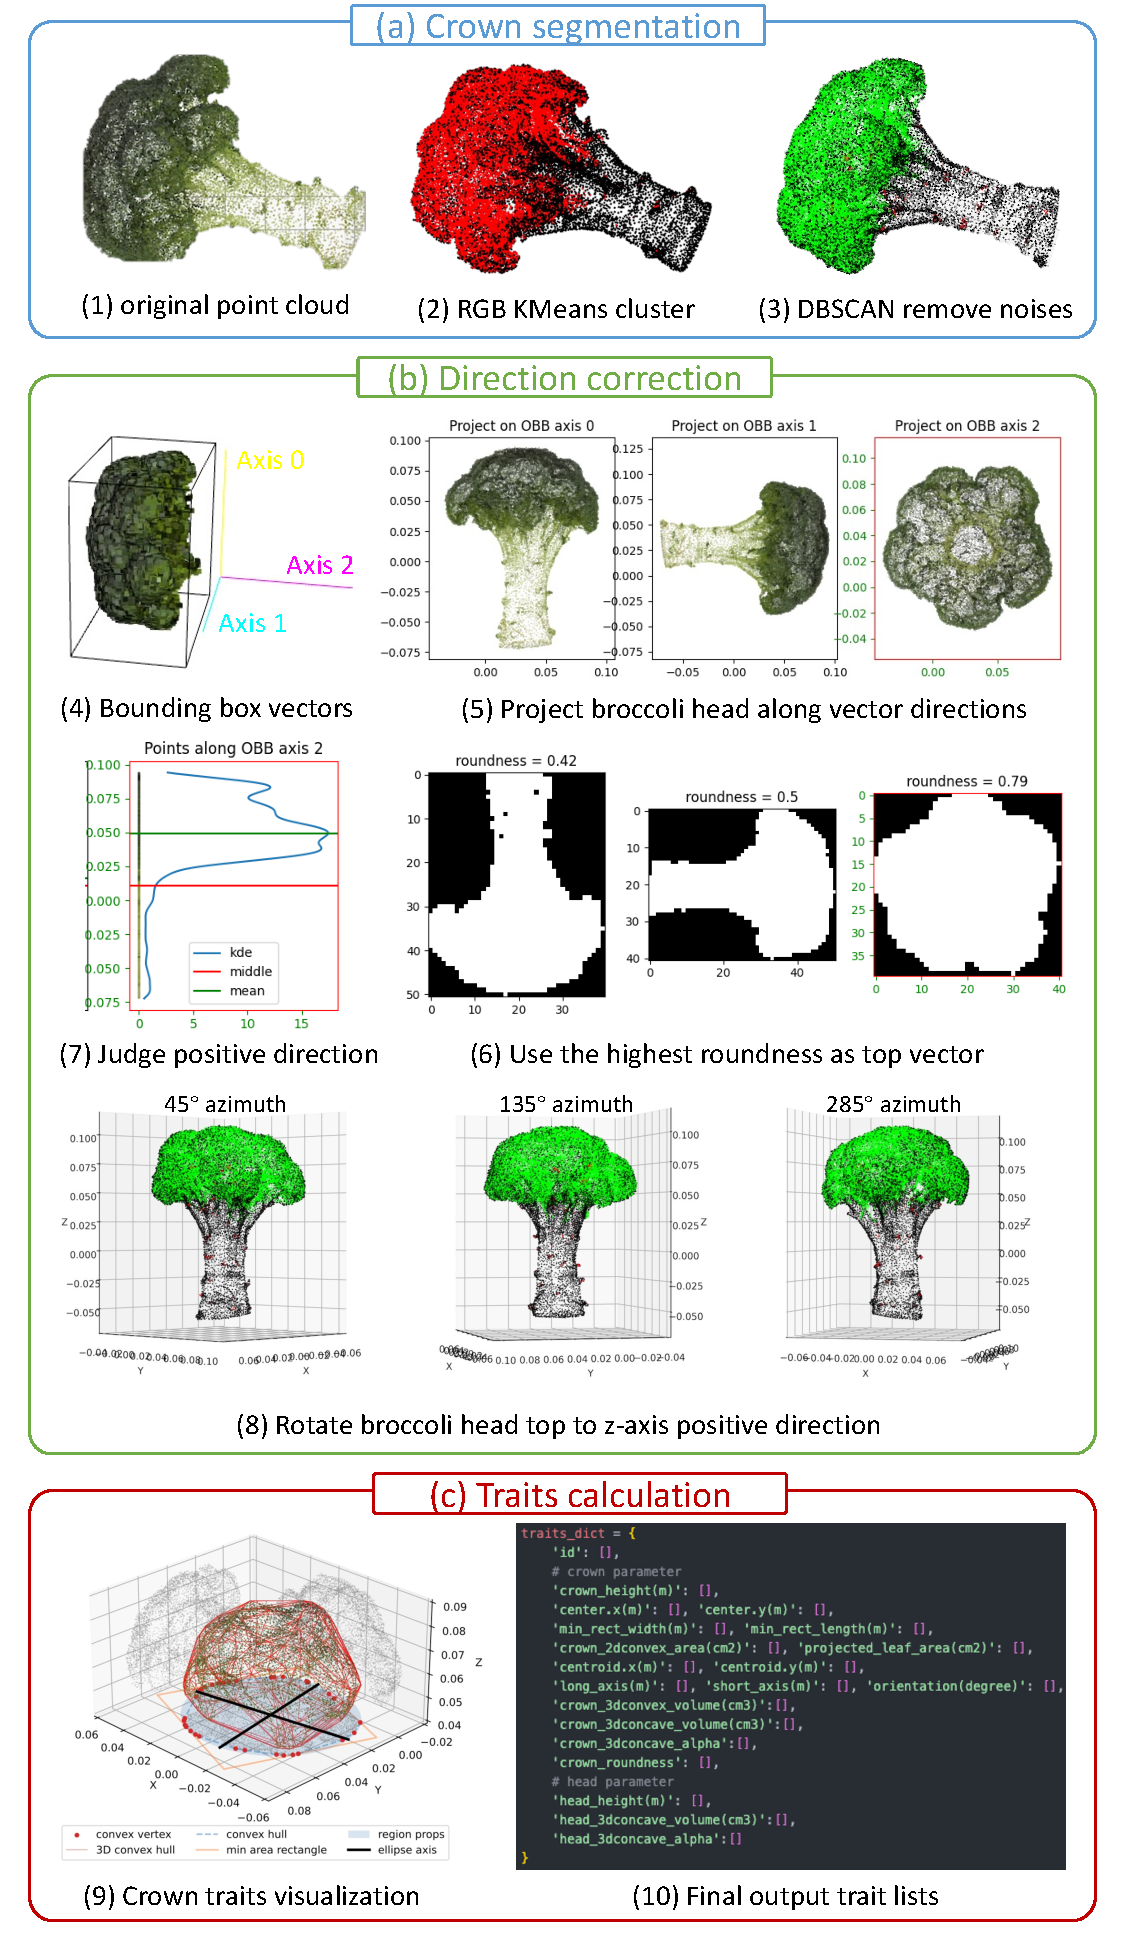
\includegraphics{figures/des/seg_algorithm.pdf}
    }
  \end{center}
  \caption[The algorithms for plant 3D model analysis]{
    The algorithms for plant 3D model analysis; (a) crown segmentation, to split the broccoli crown part and the stem part; (b) direction correction, to rotate the broccoli vertically to the z-axis positive direction; and (c) traits calculation.
  }
  \label{fig:des_seg_alg}
\end{figure}

\subsubsection{Head segmentation}

\subsubsection{Upward direction correction}

\subsubsection{Traits calculation}


\subsection{Validation}

% field measurmenet

% r2 and rmse


\section{Results}

\subsection{Image preprocessing}

% figure4: unet + casadePSP results
% add more examples
\begin{figure}[htb]
  \begin{center}
    \resizebox{\textwidth}{!}{
      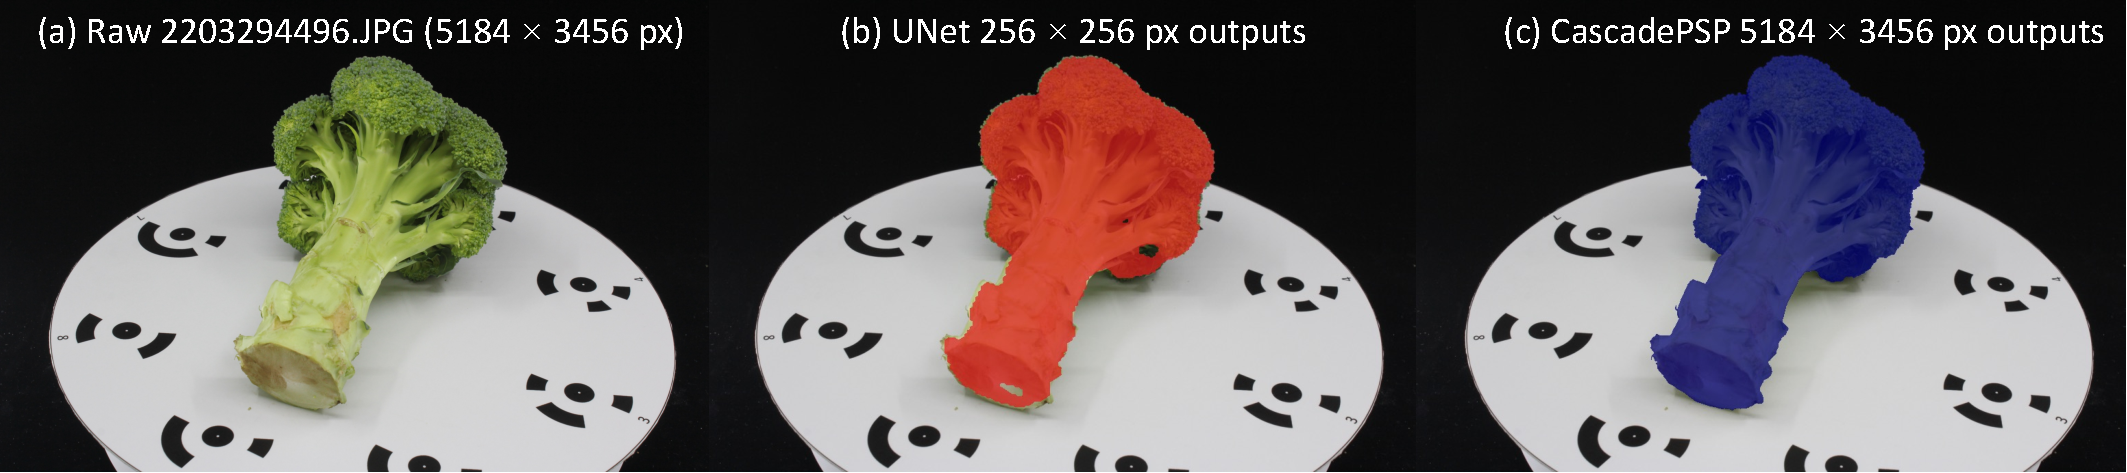
\includegraphics{figures/des/dl_seg.pdf}
    }
  \end{center}
  \caption[Two deep learning segmentation results]{
    An example of two deep learning segmentation results. (a) is the original image of broccoli head id ``2-11'' of rotating group 3, the resolution is $5184 \times 3456$ pixel; (b) is the output of the UNet segmentation, the resolution is $256 \times 256$ pixel, which is not enough as final plant masks; and (c) the output of the refined high-resolution mask using CasadePSP based on the UNet output. The mask has the same resolution as the original image.
  }
  \label{fig:des4}
\end{figure}

\subsection{Plant 3D model}

% figure5: comparison between real photo and photos + model 3 views
\begin{figure}[htb!]
  \begin{center}
    \resizebox{\textwidth}{!}{
      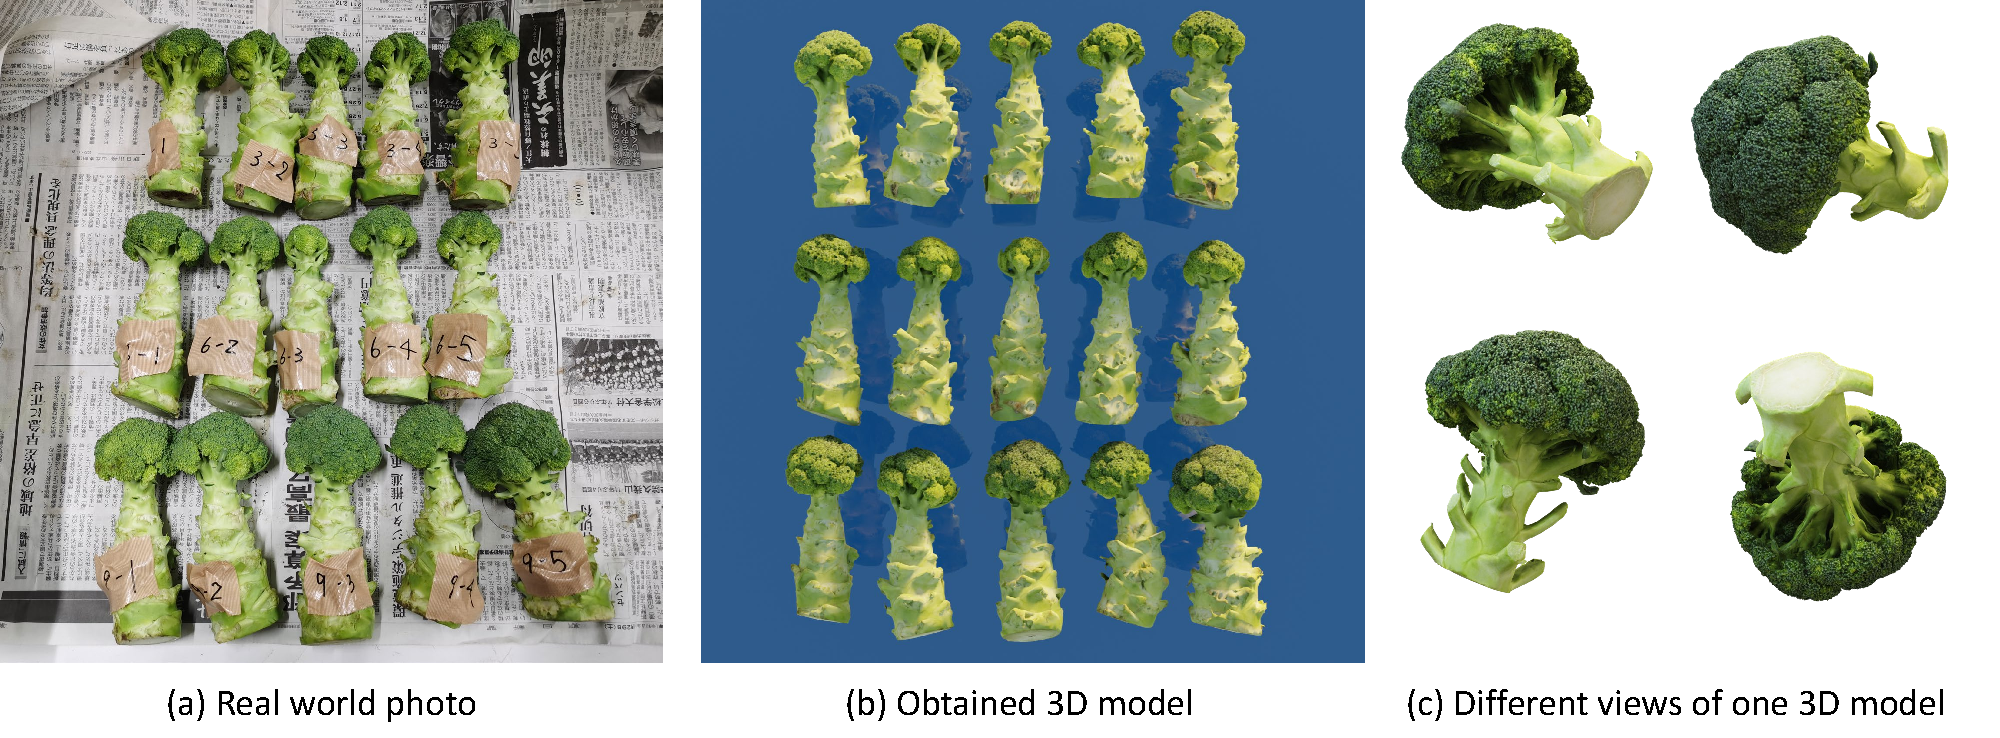
\includegraphics{figures/des/model_results.pdf}
    }
  \end{center}
  \caption[The obtained 3D models]{
    Some examples of obtained 3D models; (a) the image of 15 broccoli heads in the real world; (b) the obtained 3D models of corresponding broccoli heads; and (c) the different views of one broccoli head 3D model.
  }
  \label{fig:des_model_results}
\end{figure}

\subsection{Traits extraction}

% figure6: head extraction
% change to all reulst + one demo
\begin{figure*}[htb]
  \centering
  \begin{subfigure}[b]{0.475\textwidth}
    \centering
    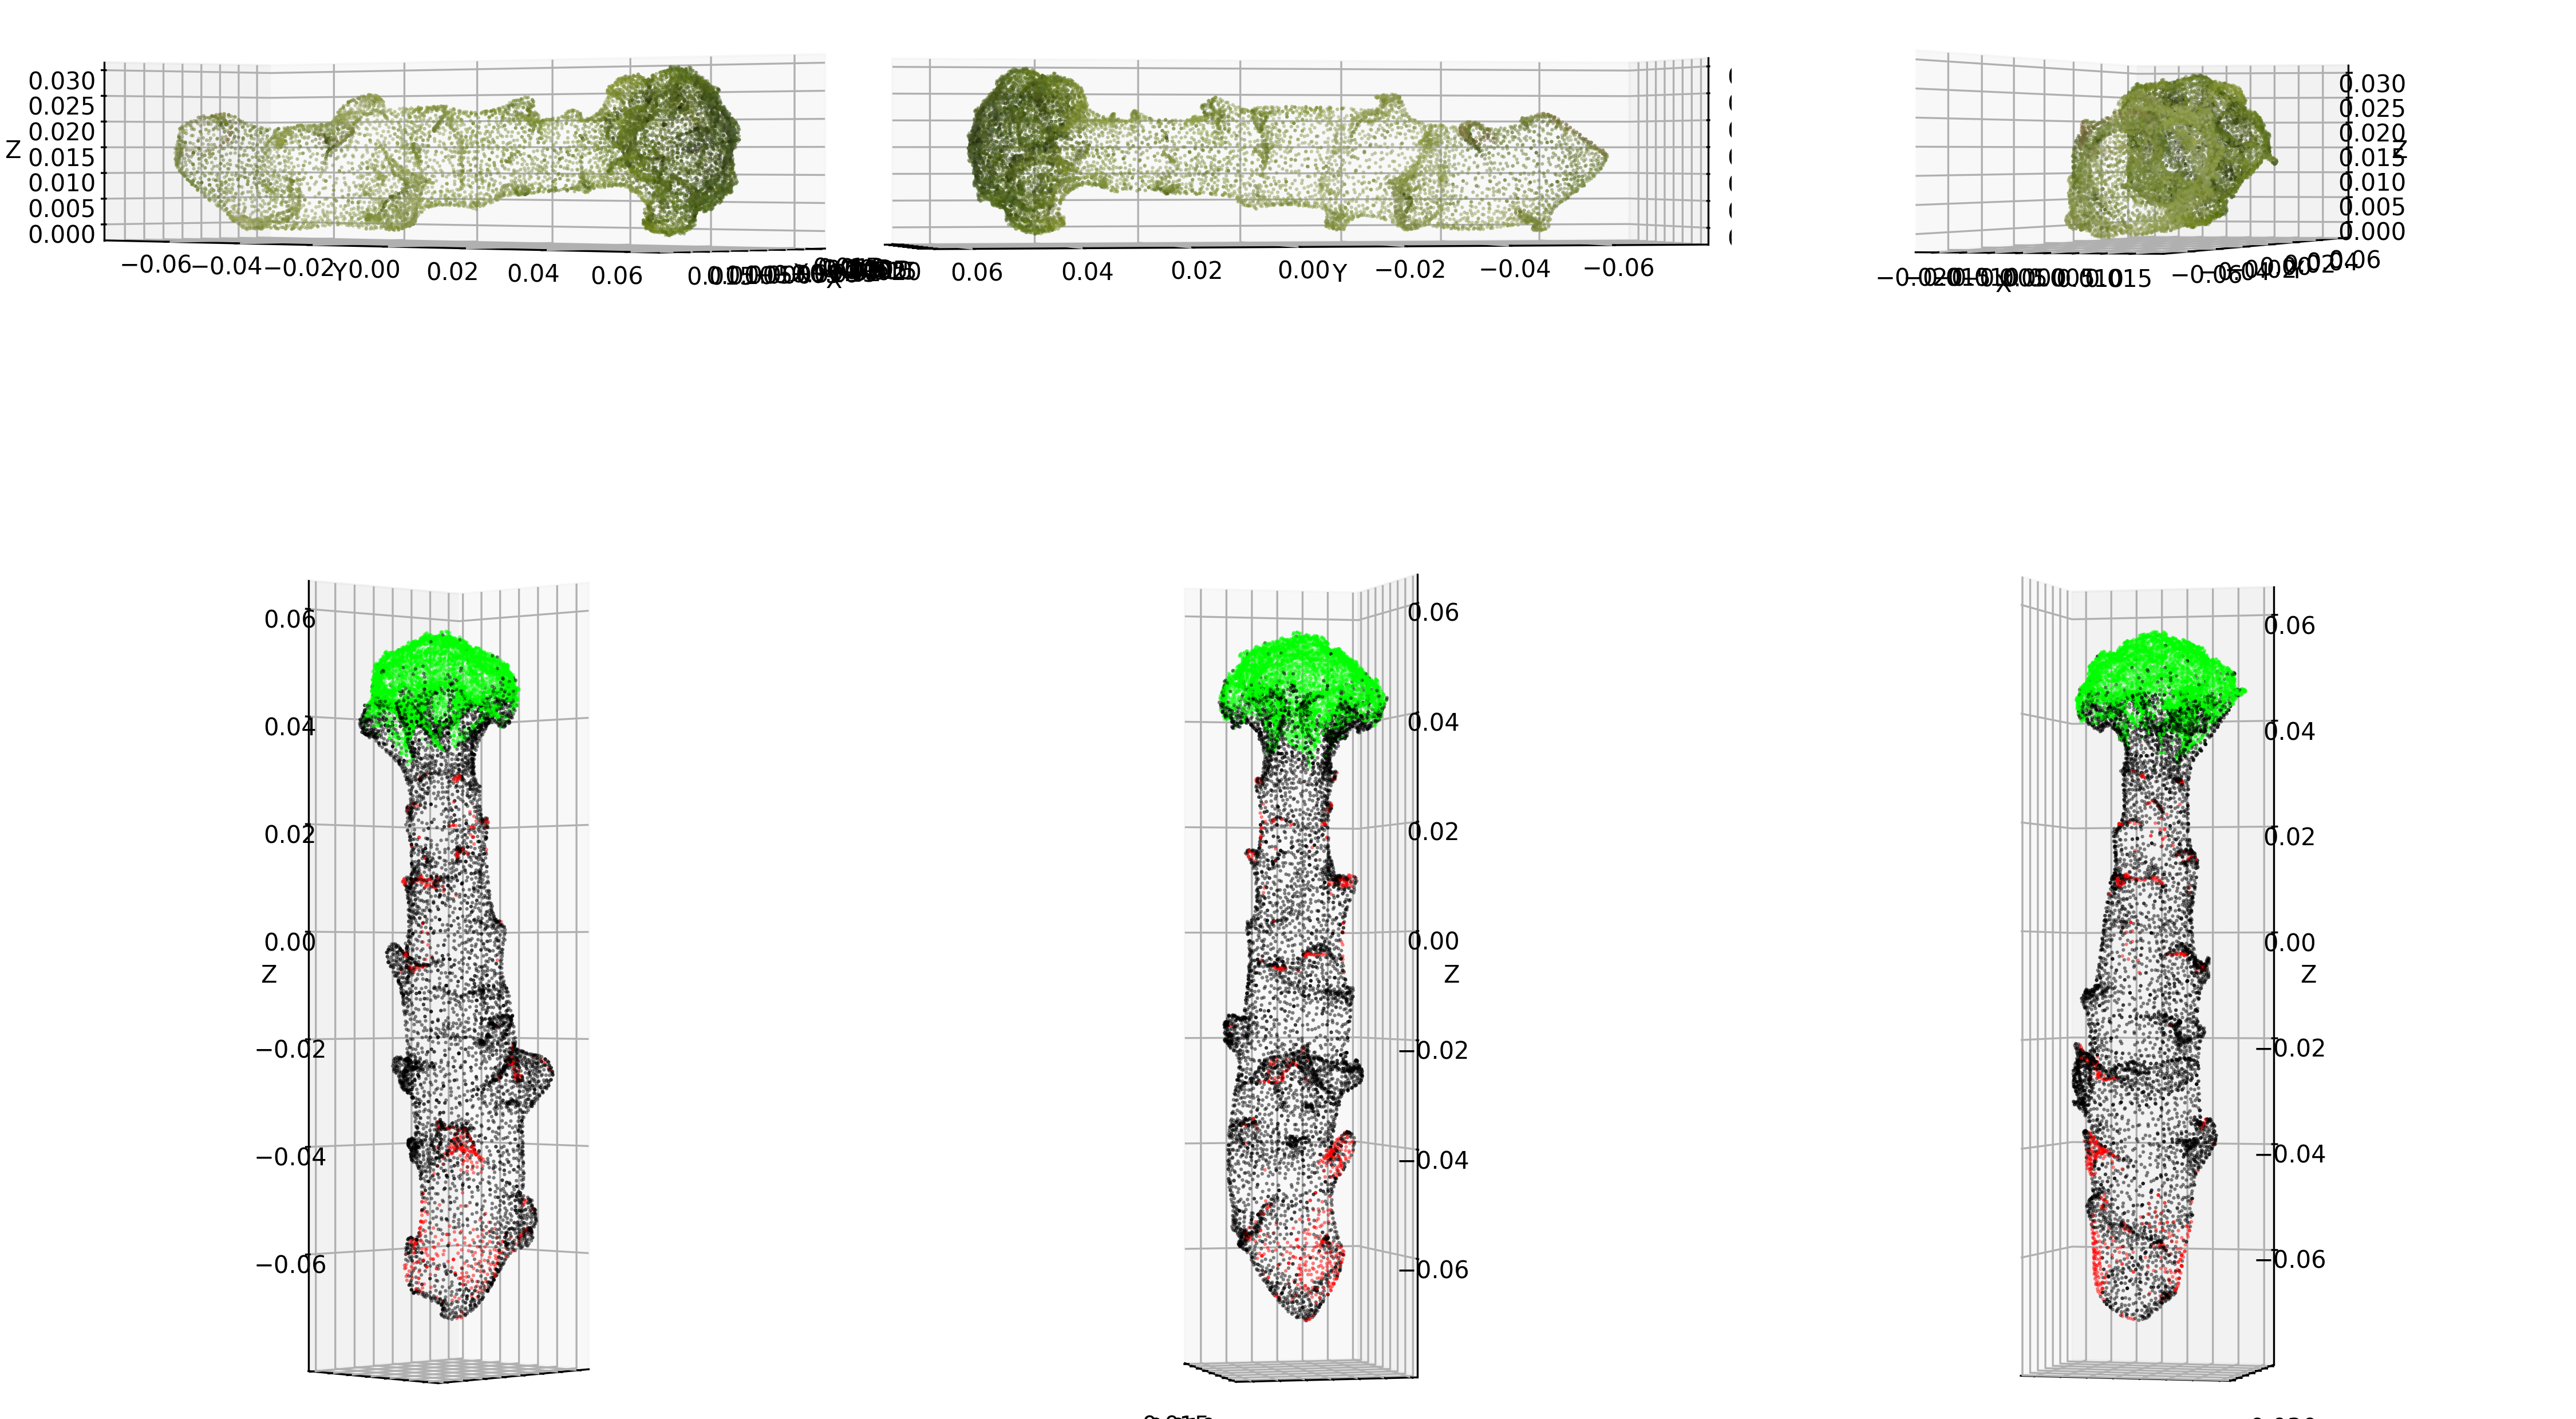
\includegraphics[width=\textwidth]{figures/des/7-2-2.png}
    \caption{ID 7-2-2}
  \end{subfigure}%
  \hfill
  \begin{subfigure}[b]{0.475\textwidth}
    \centering
    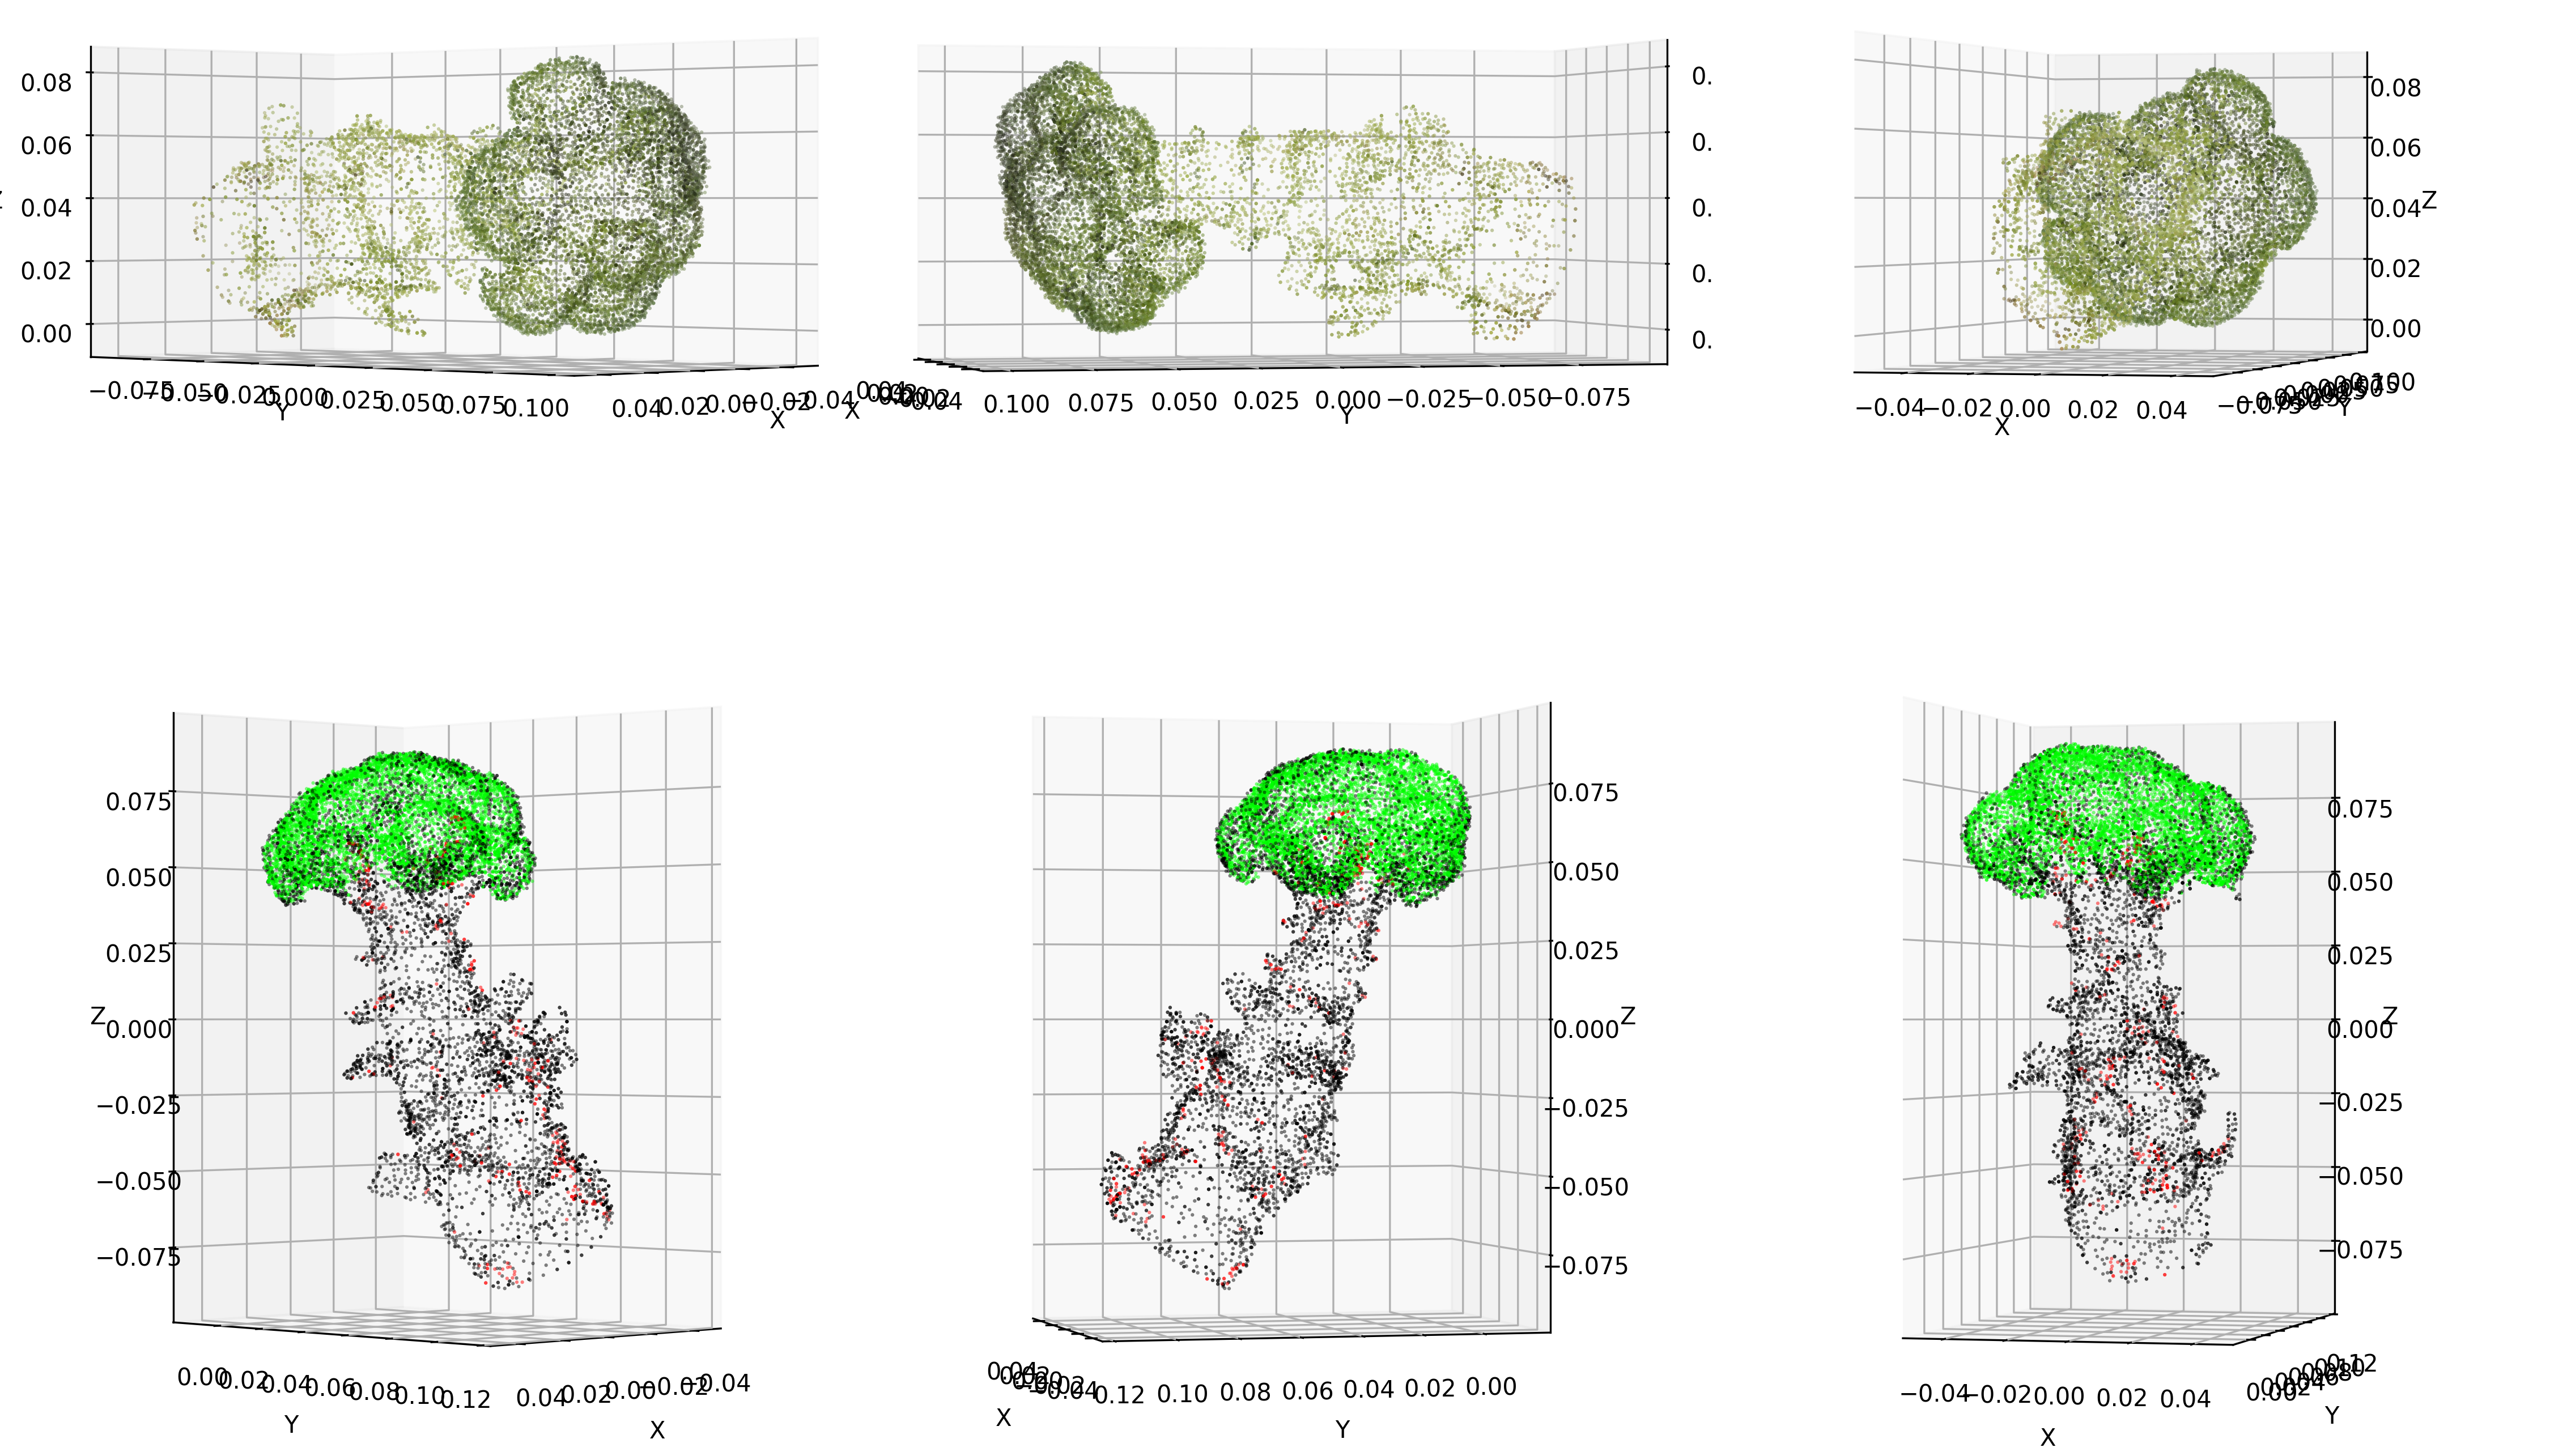
\includegraphics[width=\textwidth]{figures/des/1-5.png}
    \caption{ID 1-5}
  \end{subfigure}
  \vskip\baselineskip

  \begin{subfigure}[b]{0.475\textwidth}
    \centering
    \includegraphics[width=\textwidth]{figures/des/2-23.png}
    \caption{ID 2-23}
  \end{subfigure}%
  \hfill
  \begin{subfigure}[b]{0.475\textwidth}
    \centering
    \includegraphics[width=\textwidth]{figures/des/1-33.png}
    \caption{ID 1-33}
  \end{subfigure}%
  \caption[Examples of plant 3D model analysis at different growing stages]{
    Examples of plant 3D model analysis at different growing stages. The upper parts are the original coordinates of the obtained 3D models, while the lower parts are the segmented and direction-corrected results, the red parts are removed noises. Three columns show the corresponding azimuth angle views at $45^\circ$, $165^\circ$, and $285^\circ$ for the same 3D model.
  }
  \label{fig:des6}
\end{figure*}


\subsection{Validation}

\begin{figure}[htb!]
  \begin{center}
    \resizebox{\textwidth}{!}{
      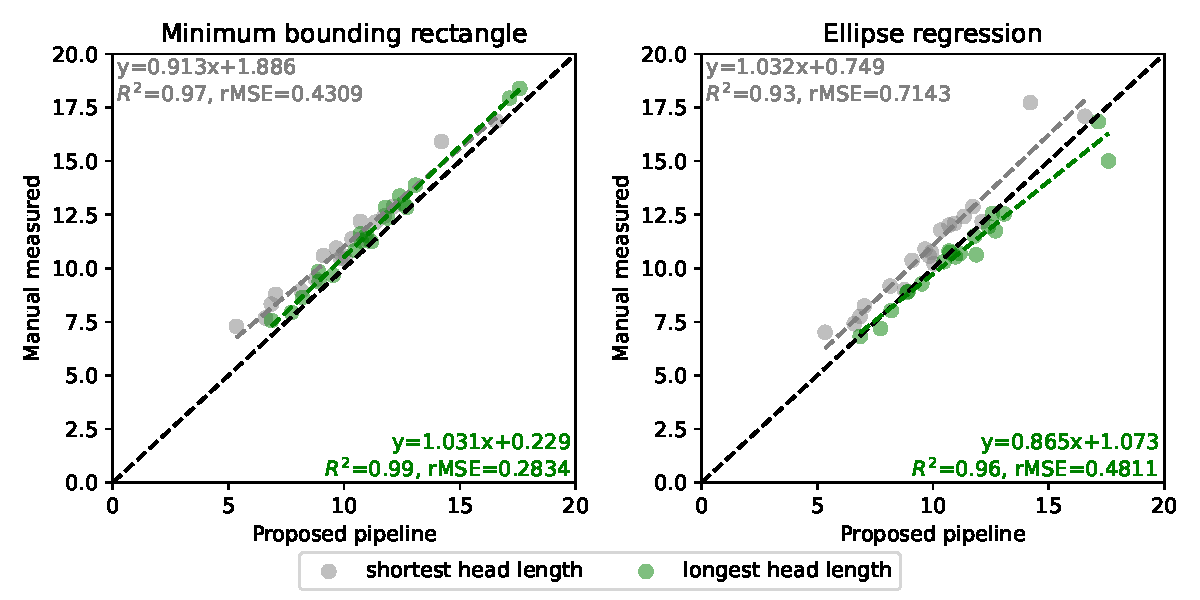
\includegraphics{figures/des/method_compare.pdf}
    }
  \end{center}
  \caption[The comparison between the proposed phenotyping pipeline and manual measurement]{
    The comparison between the proposed phenotyping pipeline and manual measurement. The shortest length and longest length of the broccoli head are compared. For the proposed pipeline, it uses two methods to estimate those lengths. One is using the length and width of the minimum bounding rectangle, the other is using the major and minor axes of the fitted ellipse.
  }
  \label{fig:des_compare}
\end{figure}

\section{Discussion}



\section{Conclusion}